\chapter{Проектирование}
\label{cha:design}

%В данном разделе реализуется новая всячина.
При разработки нового модуля было решено использовать существующие фреймворки, реализующие стандарт SAML. В данной главе приведен обзор выбранных фреймворков и произведен анализ возможности их интеграции с системой AEM. На основе выбранного фреймворка спроектирована архитектура разрабатываемого модуля. 

\section{Выбор фреймворка}
Список фреймворков, рассматриваемых при разработке, был получен с официального сайта SAML \cite{web:samlFrameworksOasis} и со страницы в википедии \cite{web:samlFrameworksWiki}. Поскольку AEM основана на Java были выбраны только совместимые с системой фреймворки. 

\subsection{Обзор выбранных фреймворков}
Для сравнения выбранных фреймворков была составлена таблица 2.1, в которой выполняется сравнение по следующим параметрам:

\begin{itemize}
\item Поддержка - осуществляется ли поддержка библиотеки, когда выпущена последняя версия.
\item Количество запросов на stackoverflow - количество запросов на stackoverflow показывает насколько популярна библиотека.
\item Примеры и документация - наличие примеров и документации.
\end{itemize}

\begin{longtable}{|p{3cm}|p{47mm}|p{30mm}|p{35mm}|}
  \caption{Сравнение SAML фреймворков}
  \label{tab:tabular}
  \\ \hline
  Название & Поддержка & Количество запросов на stackoverflow & Примеры и документация \\
  \hline \endfirsthead
  \subcaption{Продолжение таблицы~\ref{tab:tabular}}
  \\ \hline \endhead
  \hline \subcaption{Продолжение на след. стр.}
  \endfoot
  \hline \endlastfoot
  OpenSAML 3  
  & Поддерживается, последняя версия: март 2017
  & 399
  & Есть примеры, книги, плохая документация на официальном сайте \\
  \hline
  OneLogin       			   
  & Поддерживается, последняя версия: ноябрь 2018
  & 324
  & Есть примеры, хорошая документация на официальном сайте \\
  \hline
  Spring Security SAML                
  & Поддерживается, последняя версия: март 2019
  & боле 500
  & Есть примеры, плохая документация на официальном сайте \\
  \hline
  Pac4j       			   
  & Поддерживается, последняя версия: февраль 2019
  & 16
  & Есть примеры, хорошая документация на официальном сайте \\
  \hline
\end{longtable}	

Составленная таблица не позволяет однозначно сказать какое решение подойдет лучше всего, поэтому с использованием каждого фреймворка был разработан прототип приложения, формирующий сообщение авторизации с заданным параметрами-заглушками, пример сообщения приведен в листинге \ref{lst:authnRequestExample}. Разработанные прототипы позволят сравнить возможности настройки фреймворков, удобство использования и доработок под свои нужны.

\begin{longlisting}
\inputminted[linenos,frame=single]{xml}{inc/src/authnRequestExample}
\caption{Пример SAML AuthnRequest} 
\label{lst:authnRequestExample}
\end{longlisting}

\subsection{Интеграция фреймворков с AEM}
При попытке интеграции разработанных прототипов со средой AEM все прототипы оказались не работоспособны. В результате анализа было выявлено что это частое явление при использование сторонних библиотек не оптимизированных для работы в среде OSGI \cite{web:usingClassLoaders}.

Данная проблема возникает из-за различий в загрузки классов классического Java приложения и среды OSGI. В классическом Java приложении существует один загрузчик классов на все приложение, в среде OSGI для каждого модуля существует свой загрузчик классов. Все фреймворки используют для загрузки классов контекст который не знает о существование среды OSGI, листинг \ref{lst:threadContext}, и поэтому происходит ошибка при загрузки файлов. Для решения данной проблемы необходимо переопределить код фреймворка, который отвечает за загрузку классов.

\begin{listing}[H]
\inputminted[linenos,frame=single]{java}{inc/src/threadContext}
\caption{Загрузчик классов не работающий в среде OSGI} 
\label{lst:threadContext}
\end{listing}

\subsection{Заключение}
Составленная таблица и разработанный прототип позволили подробно изучить фреймворки и выделить плюсы и минусы их использования при разработки. Ниже приведены выводы по каждому фреймворку:

\begin{itemize}
\item OpenSAML 3 - Наиболее соответствующая стандарту реализация. Низкоуровневый фреймворк который отвечает только за формирование XML сообщений. Активно развивается и поддерживается. Требуется переопределение стартовой конфигурации так как не предназначен для работы в OSGI среде, однако из-за своей низкоуровневой архитектуры и модульности это не составляет труда. Имеет плохую официальную  документацию но множество примеров использования, так-же имеется печатное руководство по использованию \cite{web:openSamlBlog}.
\item OneLogin - Не предназначен для работы в OSGI среде, сложно изменить инициализацию. Работает с ограниченным набором провайдеров авторизации. Имеются подробные примеры использования на официальном сайте а также на stackoverflow.
\item Spring Security SAML - Использует внутри OpenSAML 2, выполняет оборачивание базовых методов, но не поддерживает все типы сообщений доступные в стандарте. Используется устаревшая версия OpenSAML 2. Плохо совместим с OSGI средой. Поддерживает большинство популярный провайдеров идентификации. Имеет большое количество примеров использования.
\item Pac4j- Использует внутри OpenSAML3, оборачивает базовые методы что позволяет реализовывать функции гораздо быстрее. Ограничен в доступных методах и настройках. Не предназначен для работы в OSGI среде. В отличие от OpenSAML 3 инициализация не может быть легко изменена что делает библиотеку не удобной в использование и требует большего времени доработки.
\end{itemize}

В результате анализа было принято решение разрабатывать модуль с применением фреймворка – OpenSAML 3. Несмотря на то что другие фреймворки предоставляют больше готовых решений они не реализуют все возможности стандарта и имеют трудности при интеграции со средой AEM.

\section{Проектные решения}
На основе требований и выбранного фреймворка можно спроектировать структуру разрабатываемого модуля. Поскольку Open SAML 3 является низкоуровневым фреймворком и в основном необходим для генерации XML сообщений было принято решение выделить следующую структуру пакетов модуля:

\begin{enumerate}
\item authentication - принимает запросы на аутентификацию и ответы от провайдера авторизации, обрабатывает и определяет их тип. Отправляет запросы к провайдеру авторизации вместе с составленными сообщениями. Сохраняет сессию пользователя в куки. Пакет имеет следующую структуру рис.~\ref{fig:coreAuthn}:
\begin{enumerate}
\item security.ecryption - пакет содержащий функции шифрования и дешифрования строк.
\item servlets - пакет содержащий сервлеты обрабатывающие запросы а также обработчики сообщений.
\item utils - пакет утилит.
\item models - пакет моделей пользователя и куки.
\end{enumerate}
\item saml - генерирует SAML сообщения с использованием выбранного фреймворка, выполняет валидацию принятых сообщений, а также выполняет настройку библиотеки при установке в систему. Имеет пакет конфигурации, который позволяет использовать проектируемый модуль во всех системах AEM с различными настройками поставщика сервиса. Пакет имеет следующую структуру рис.~\ref{fig:coreSaml}:
\begin{enumerate}
\item bundle - выполняет конфигурацию модуля при его установки в OSGI среду.
\item validator - содержит классы выполняющие валидацию утверждений полученных от IdP.
\item messages - содержит классы работы с сообщениями авторизации.
\item configuration - содержит конфигурации модуля.
\item security - содержит классы извлекающие сертификаты из Java хранилища ключей и осуществляющие подпись всех XML сообщений.
\item utils - пакет утилит, необходимый для первоначальной настройки Open SAML 3 фреймворка.
\end{enumerate}
\item ids.configuration - вспомогательный пакет, не относящийся к работе напрямую но созданный в связи с дополнительными требованиями полученными в процессе разработки. Содержит конфигурацию которая задает параметры IdP и JavaScript который позволяет пользователю проходить авторизацию на стороне сайта или портала без перехода на сайт IdP.
\end{enumerate}		

\begin{figure}[h]
  \centering
  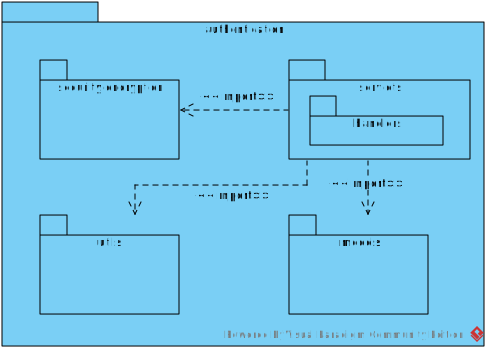
\includegraphics[width=\textwidth]{inc/svg/coreAuthn}
  \caption{Диаграмма структуры пакета authentication}
  \label{fig:coreAuthn}
\end{figure}

\begin{figure}[H]
  \centering
  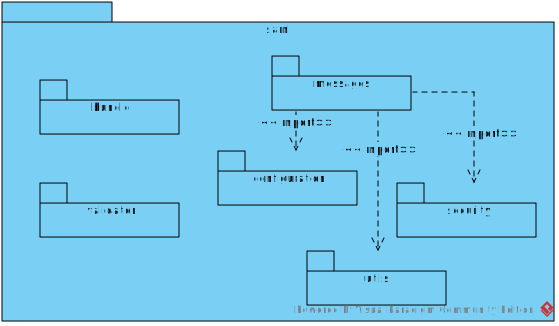
\includegraphics[width=\textwidth]{inc/svg/coreSaml}
  \caption{Диаграмма структуры пакета saml}
  \label{fig:coreSaml}
\end{figure}

\section{Заключение}
В данной главе был выбран фреймворк реализующий стандарт SAML с использованием которого будет разработан модуль. На основе выбранного фреймворка была спроектирована архитектура разрабатываемого модуля.

%%% Local Variables:
%%% mode: latex
%%% TeX-master: "rpz"
%%% End:
